% The seven bridges of Königsberg
% Author : Alain Matthes
% Encoding : UTF8
% Engine : PDFLaTeX
\documentclass[]{article}
\usepackage[utf8]{inputenc} 
\usepackage{fullpage}
\usepackage{fourier}
\usepackage{tikz}
%%%<
\usepackage{verbatim}
%\usepackage[active,tightpage]{preview}
%\PreviewEnvironment{tikzpicture}
%\setlength\PreviewBorder{5pt}%
%%%>

\begin{comment}
:Title: The seven bridges of Königsberg
:Slug: bridges-of-konigsberg

The Seven Bridges of Königsberg is a famous historical problem in mathematics.
Its negative resolution by Leonhard Euler in 1735 laid the foundations of graph theory and presaged the idea of topology.
\end{comment}

\usetikzlibrary{arrows,%
                shapes,positioning}
                
\thispagestyle{empty}
\begin{document}
  
  The Seven Bridges of Königsberg is a famous historical problem in mathematics. Its negative resolution by Leonhard Euler in 1735 laid the foundations of graph theory and presaged the idea of topology.
  
  Abstract graph corresponding to bridges of Königsberg 
  
\begin{center}
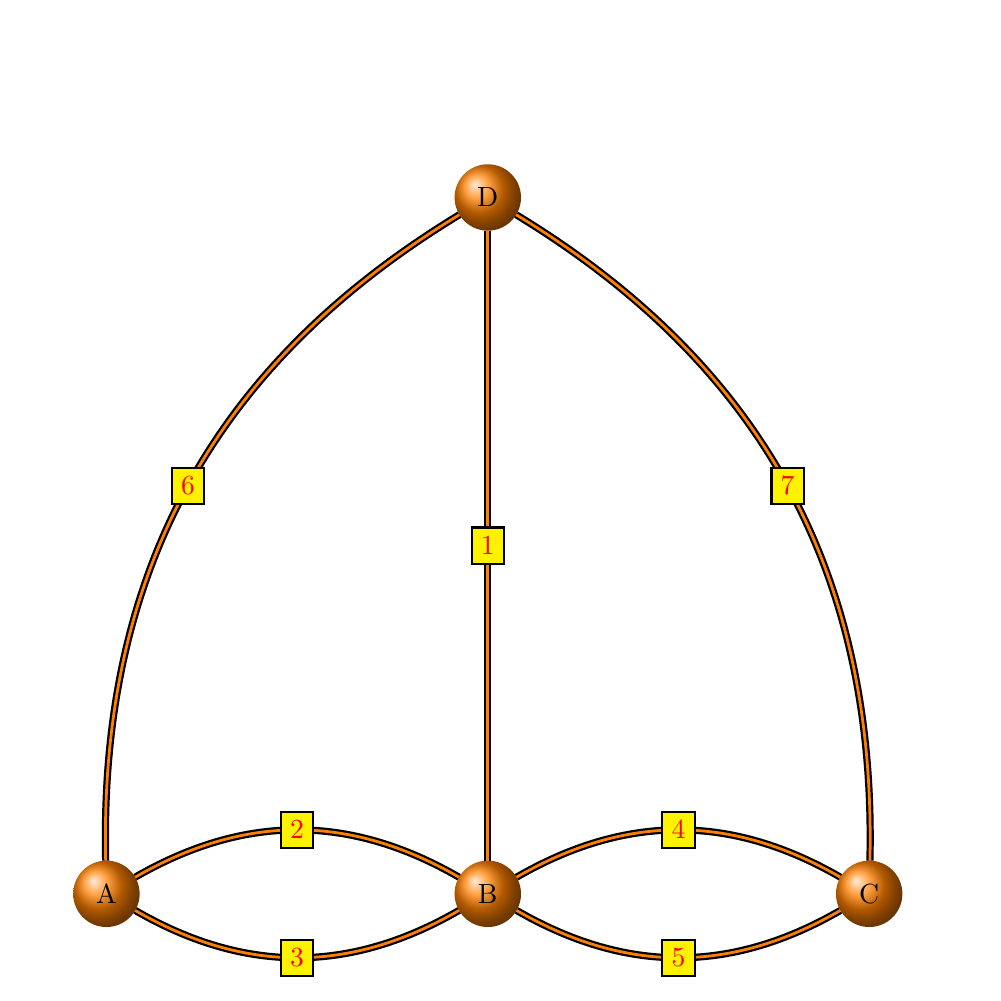
\begin{tikzpicture}[node distance   = 4 cm]
  \useasboundingbox (-1,-1) rectangle (11,11); 
  \tikzset{VertexStyle/.style = {shape          = circle,
                                 ball color     = orange,
                                 text           = black,
                                 inner sep      = 2pt,
                                 outer sep      = 0pt,
                                 minimum size   = 24 pt}}
  \tikzset{EdgeStyle/.style   = {thick,
                                 double          = orange,
                                 double distance = 1pt}}
  \tikzset{LabelStyle/.style =   {draw,
                                  fill           = yellow,
                                  text           = red}}
     \node[VertexStyle](A){A};
     \node[VertexStyle,right=of A](B){B};
     \node[VertexStyle,right=of B](C){C};
     \node[VertexStyle,above= 8 cm of B](D){D};     
     \draw[EdgeStyle](B) to node[LabelStyle]{1} (D) ;
     \tikzset{EdgeStyle/.append style = {bend left}}
     \draw[EdgeStyle](A) to node[LabelStyle]{2} (B);
     \draw[EdgeStyle](B) to node[LabelStyle]{3} (A);
     \draw[EdgeStyle](B) to node[LabelStyle]{4} (C);
     \draw[EdgeStyle](C) to node[LabelStyle]{5} (B);
     \draw[EdgeStyle](A) to node[LabelStyle]{6} (D);
     \draw[EdgeStyle](D) to node[LabelStyle]{7} (C);

  \end{tikzpicture}
\end{center}
\end{document}